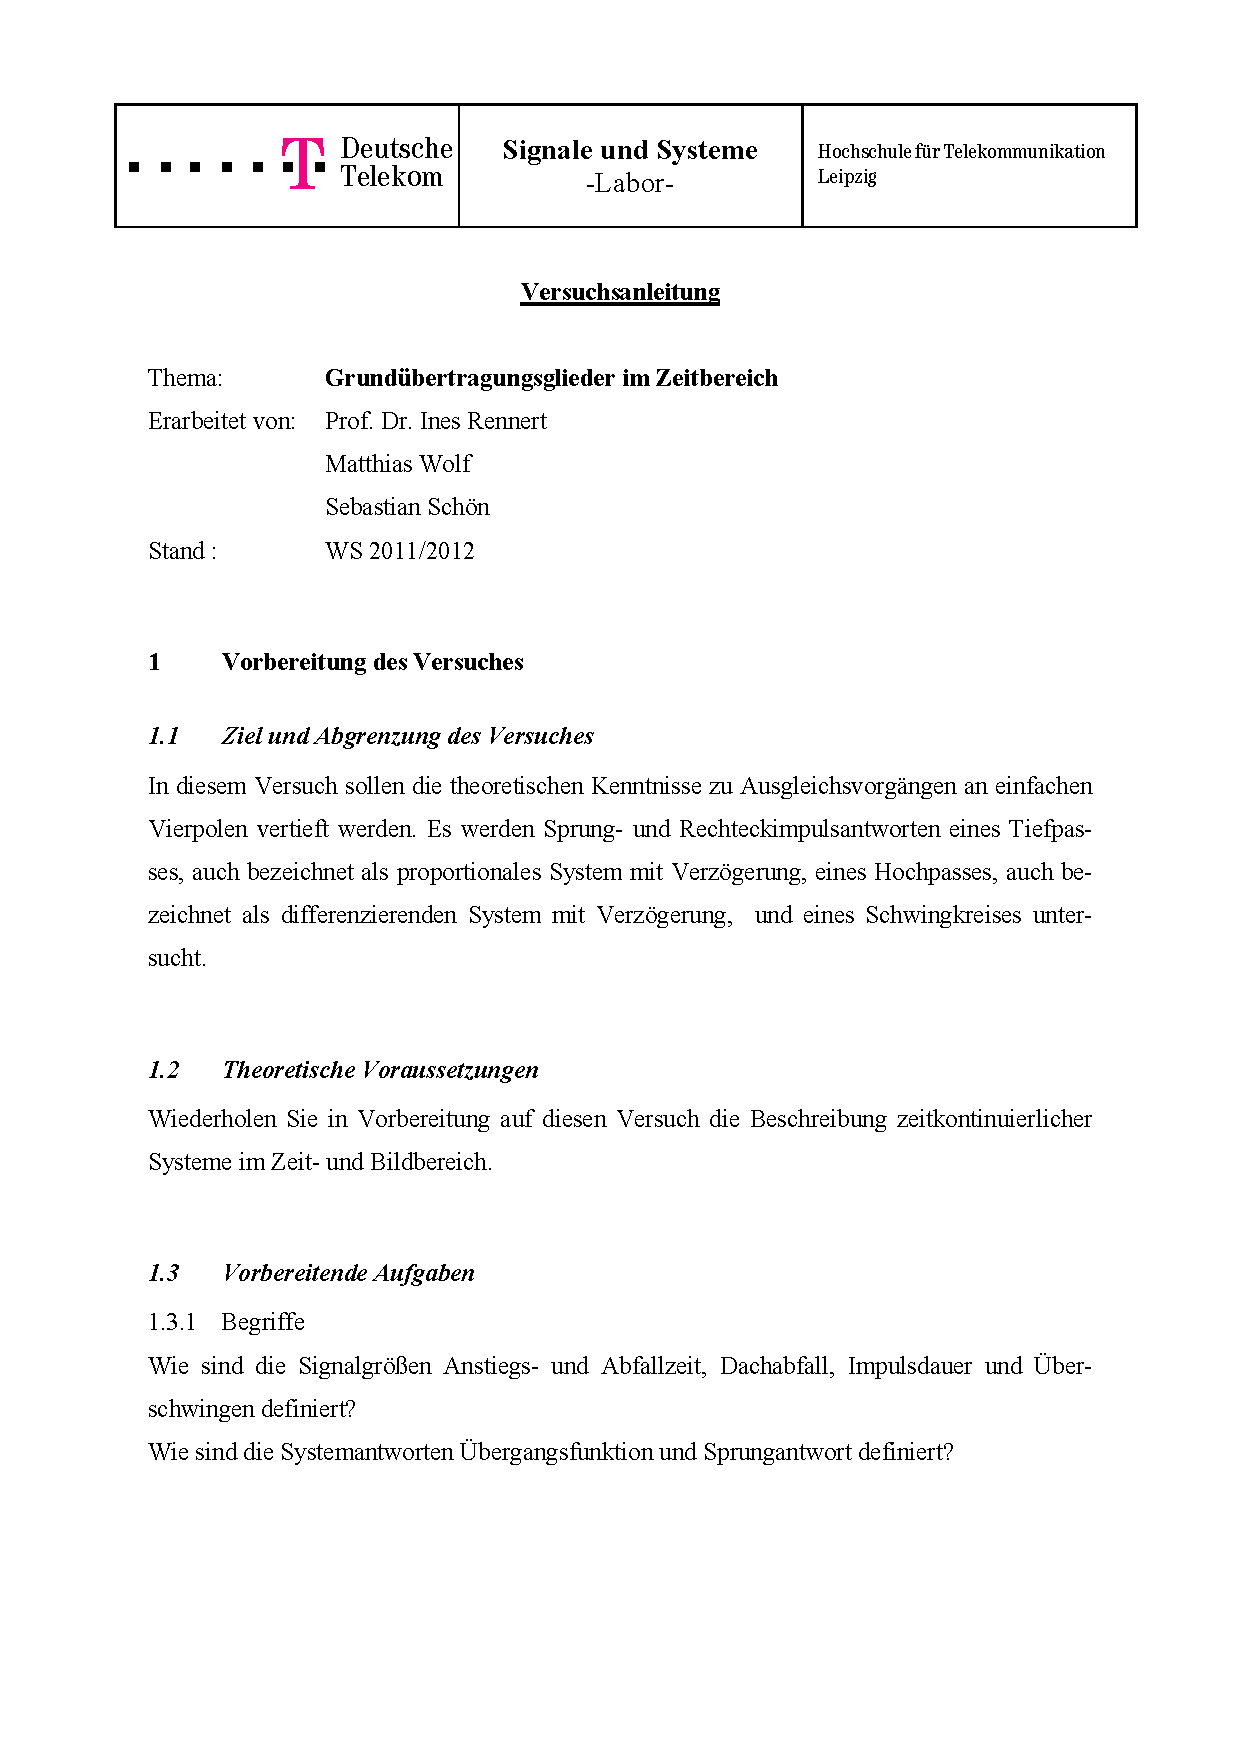
\includegraphics[width=1.0\textwidth]{Bilder/Grundubertragungsglieder im Zeitbereich (verschoben)}\newpage
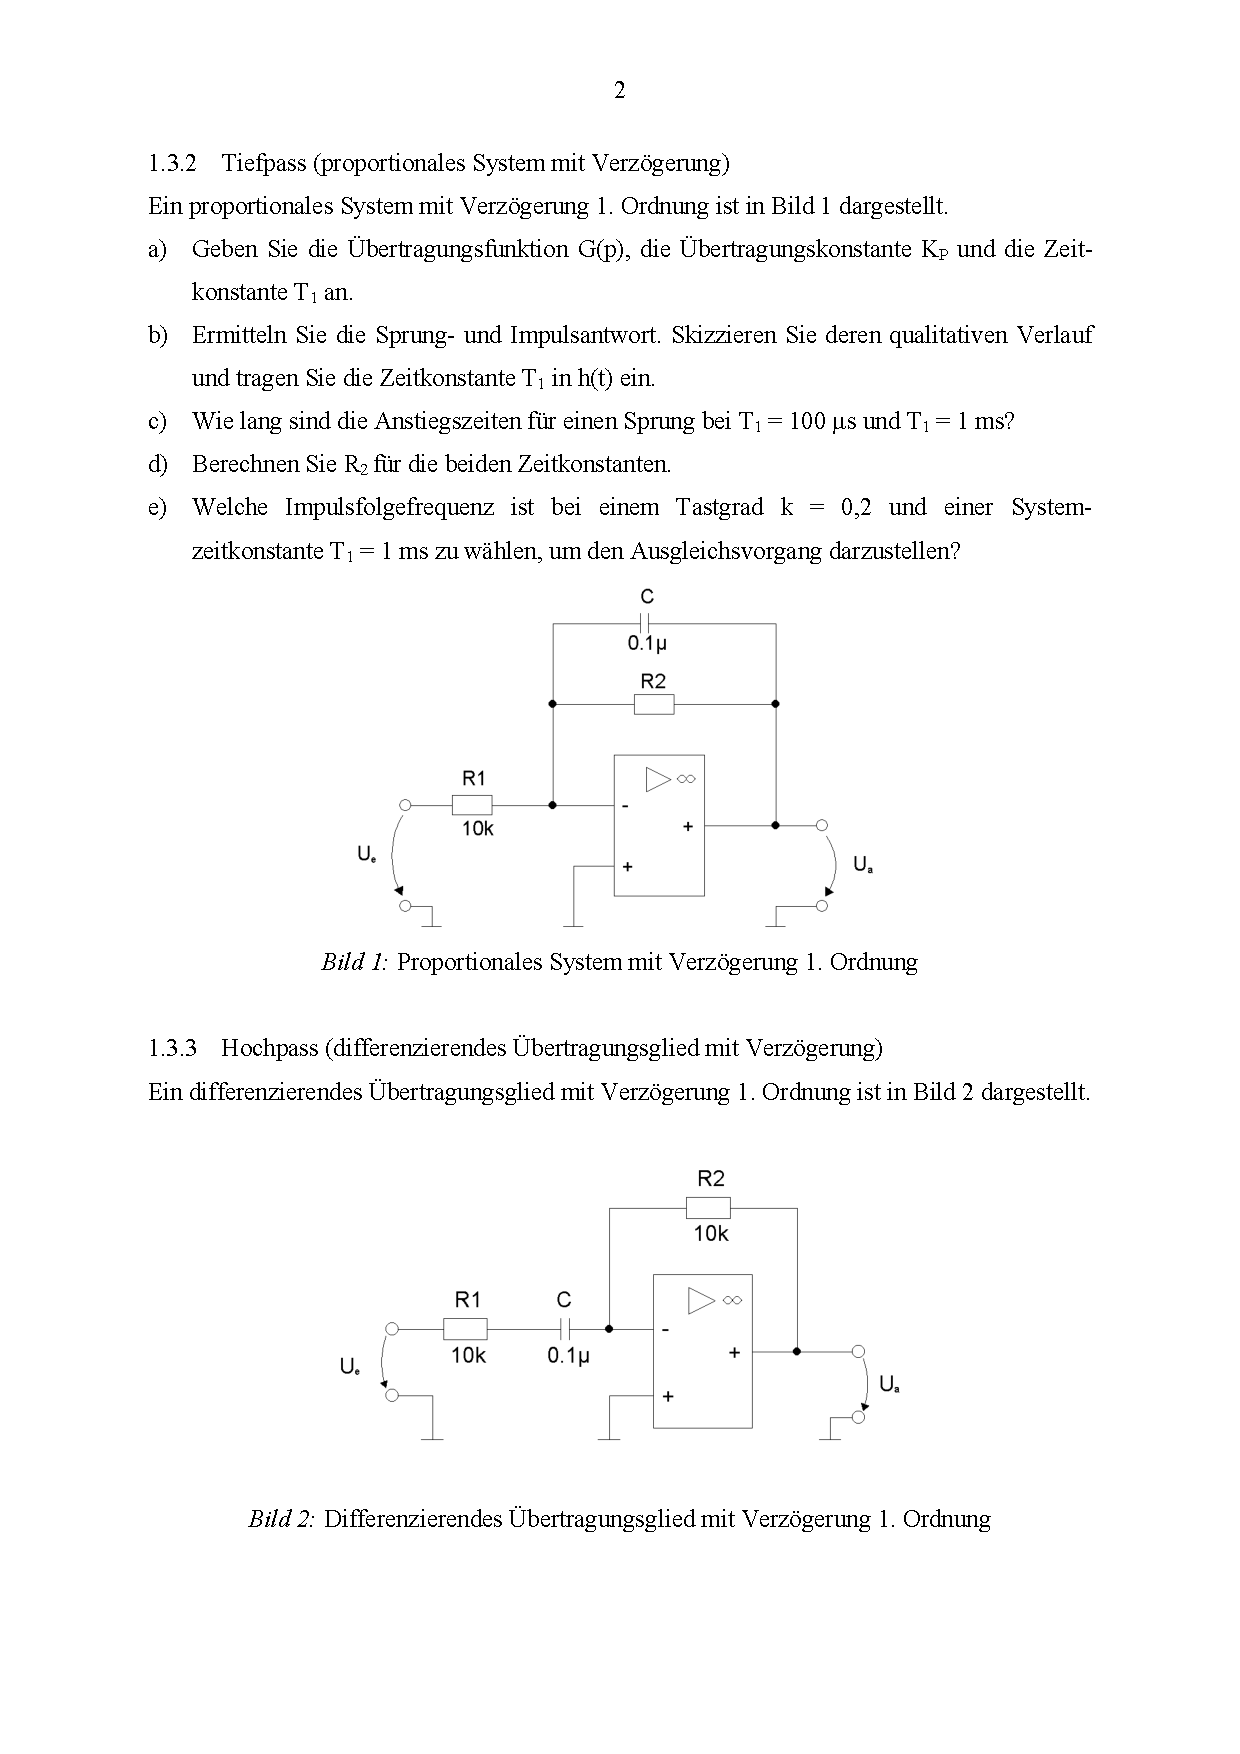
\includegraphics[width=1.0\textwidth]{Bilder/Grundubertragungsglieder im Zeitbereich (verschoben) 2}\newpage
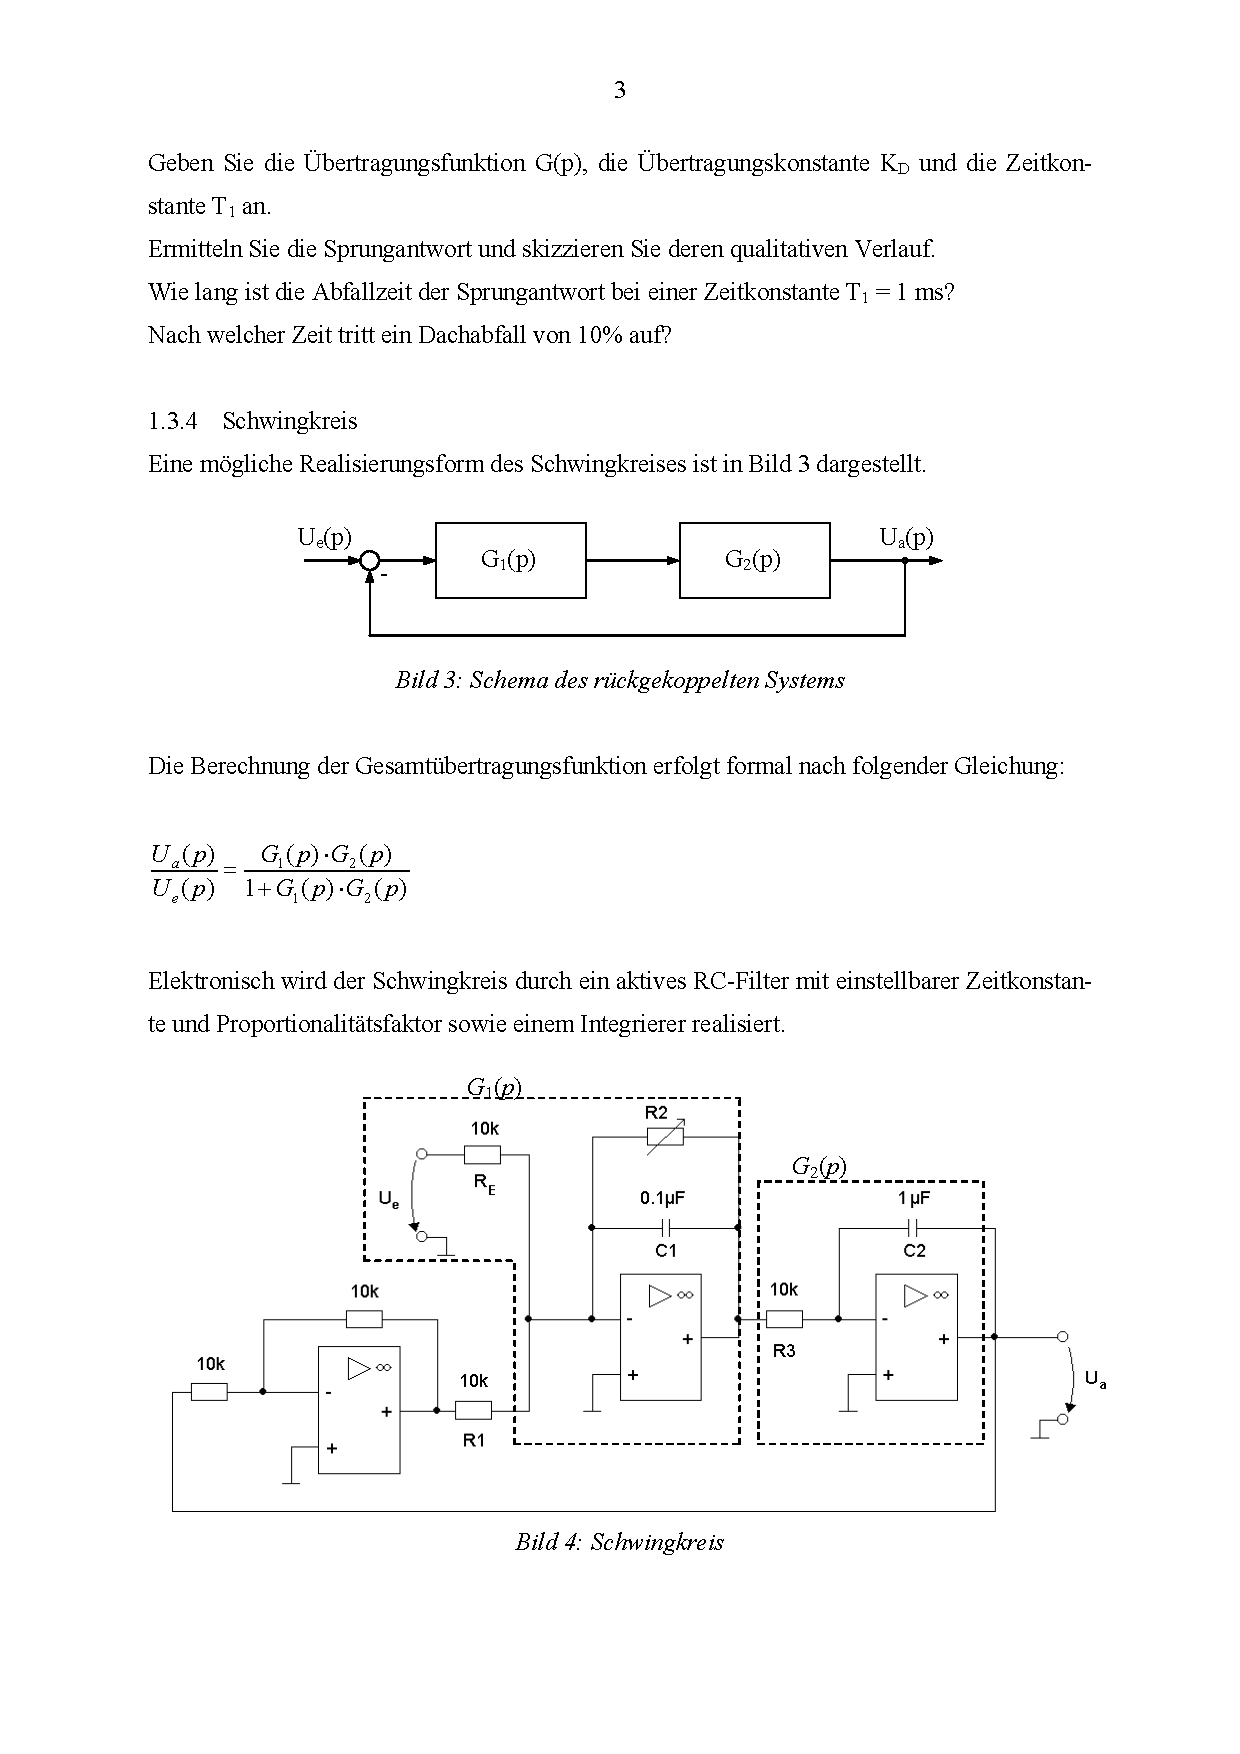
\includegraphics[width=1.0\textwidth]{Bilder/Grundubertragungsglieder im Zeitbereich (verschoben) 3}\newpage
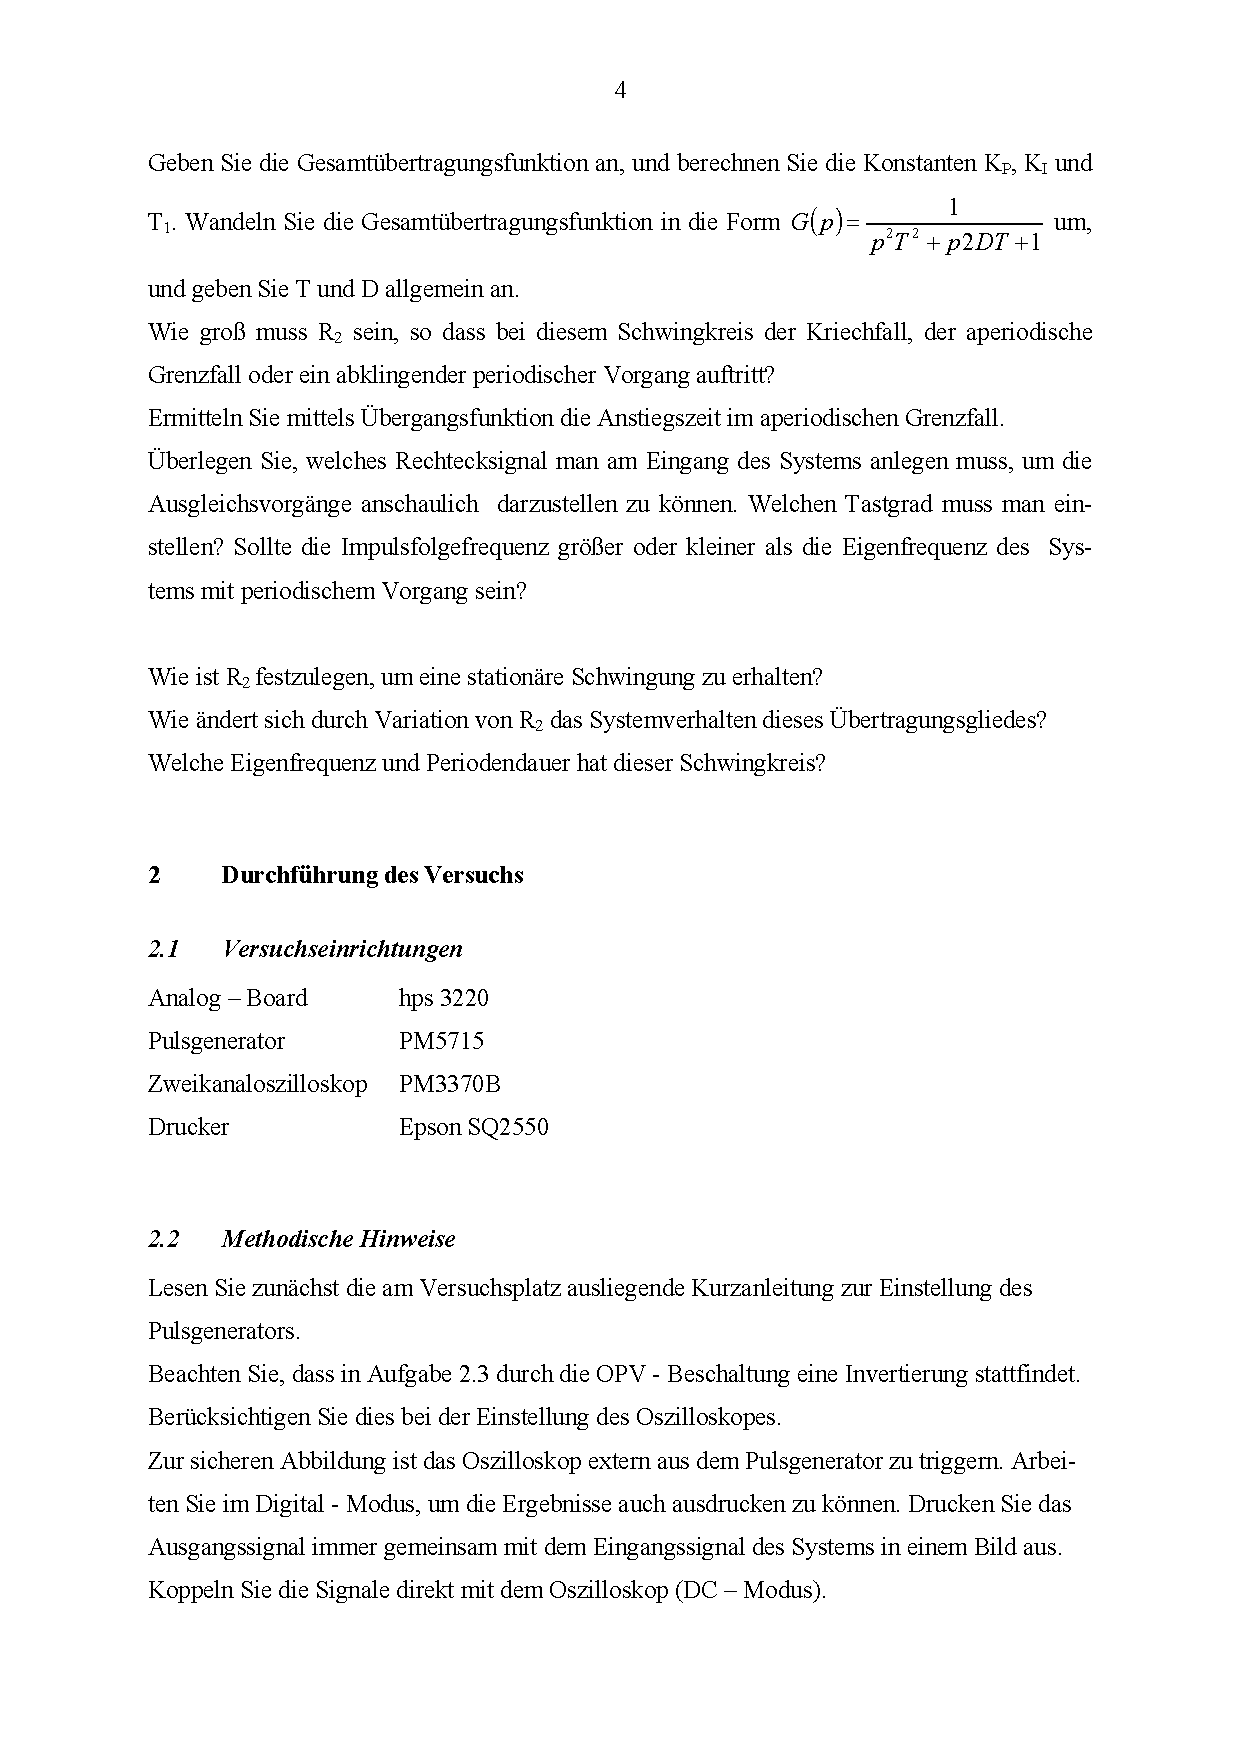
\includegraphics[width=1.0\textwidth]{Bilder/Grundubertragungsglieder im Zeitbereich (verschoben) 4}\newpage
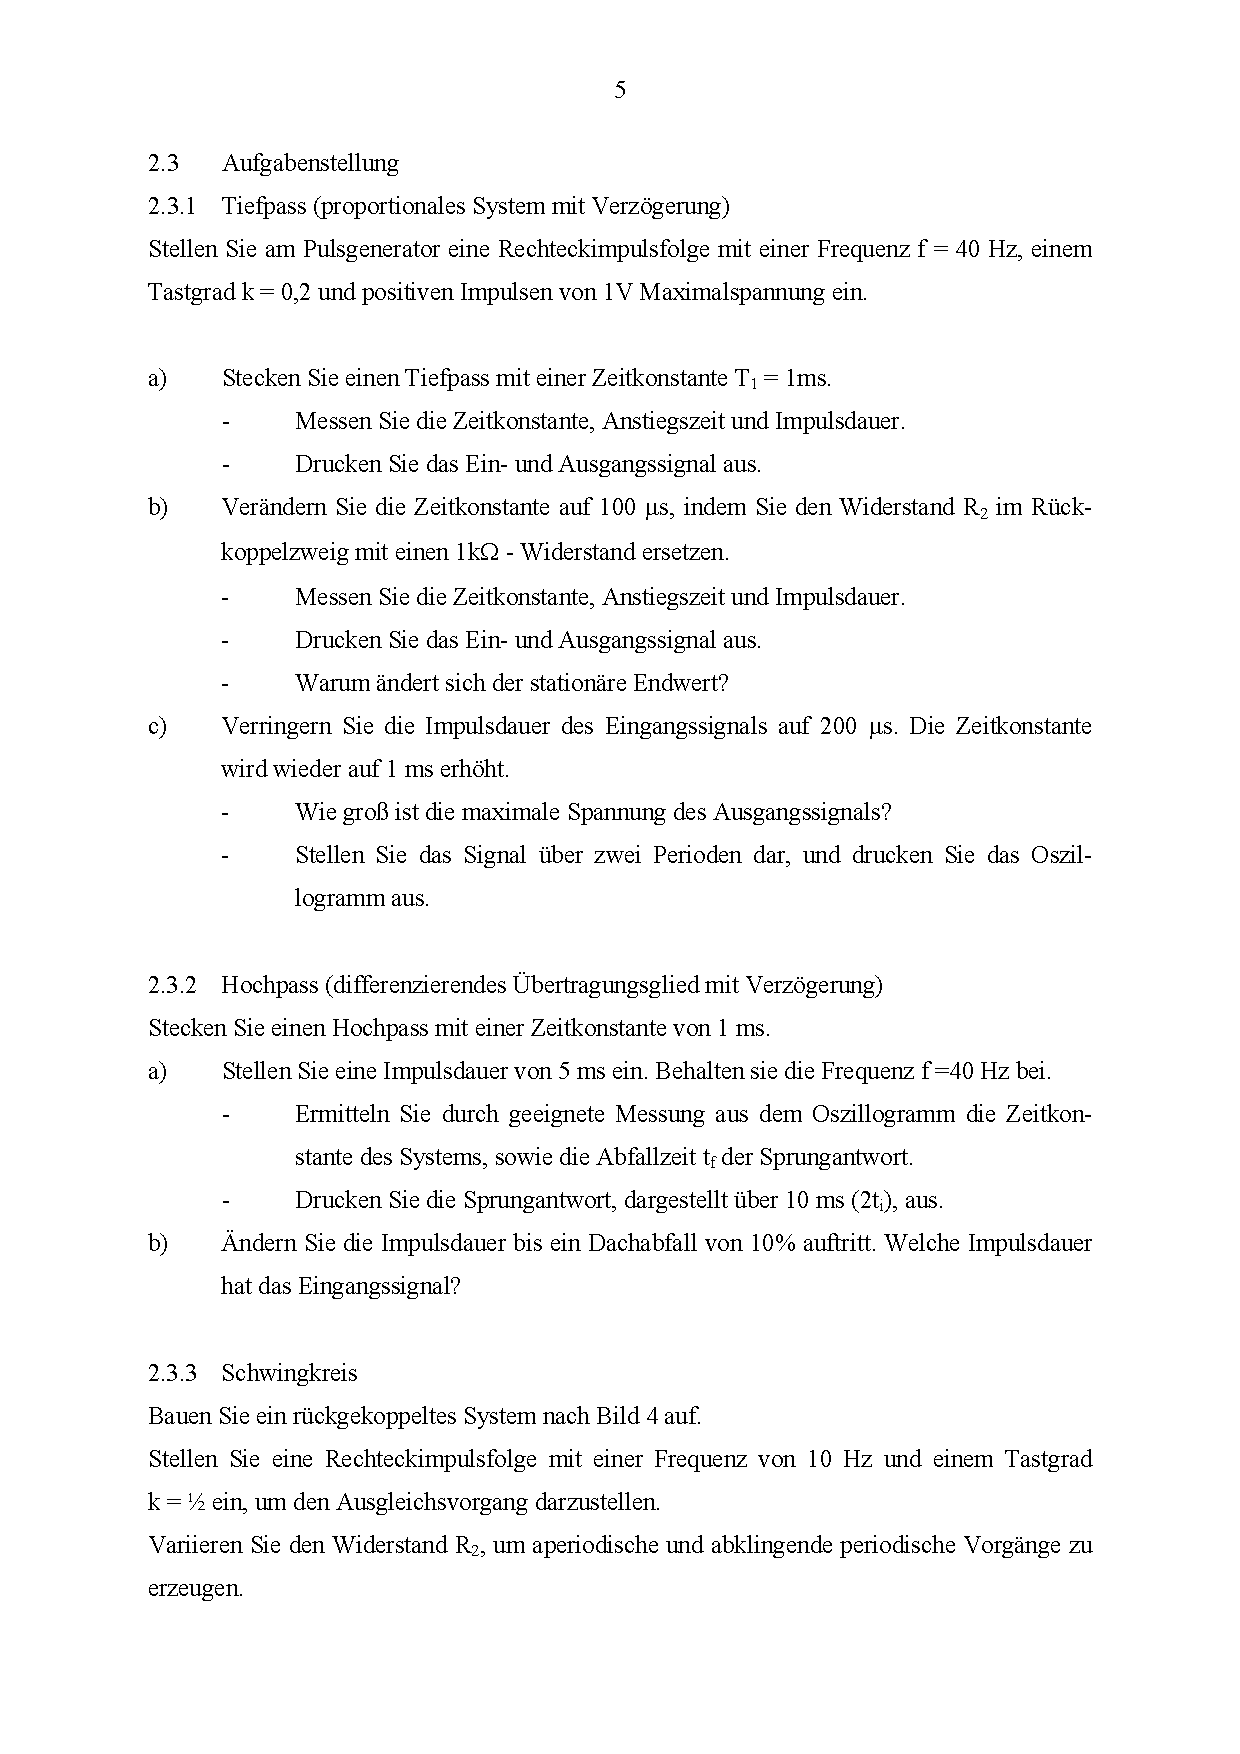
\includegraphics[width=1.0\textwidth]{Bilder/Grundubertragungsglieder im Zeitbereich (verschoben) 5}\newpage
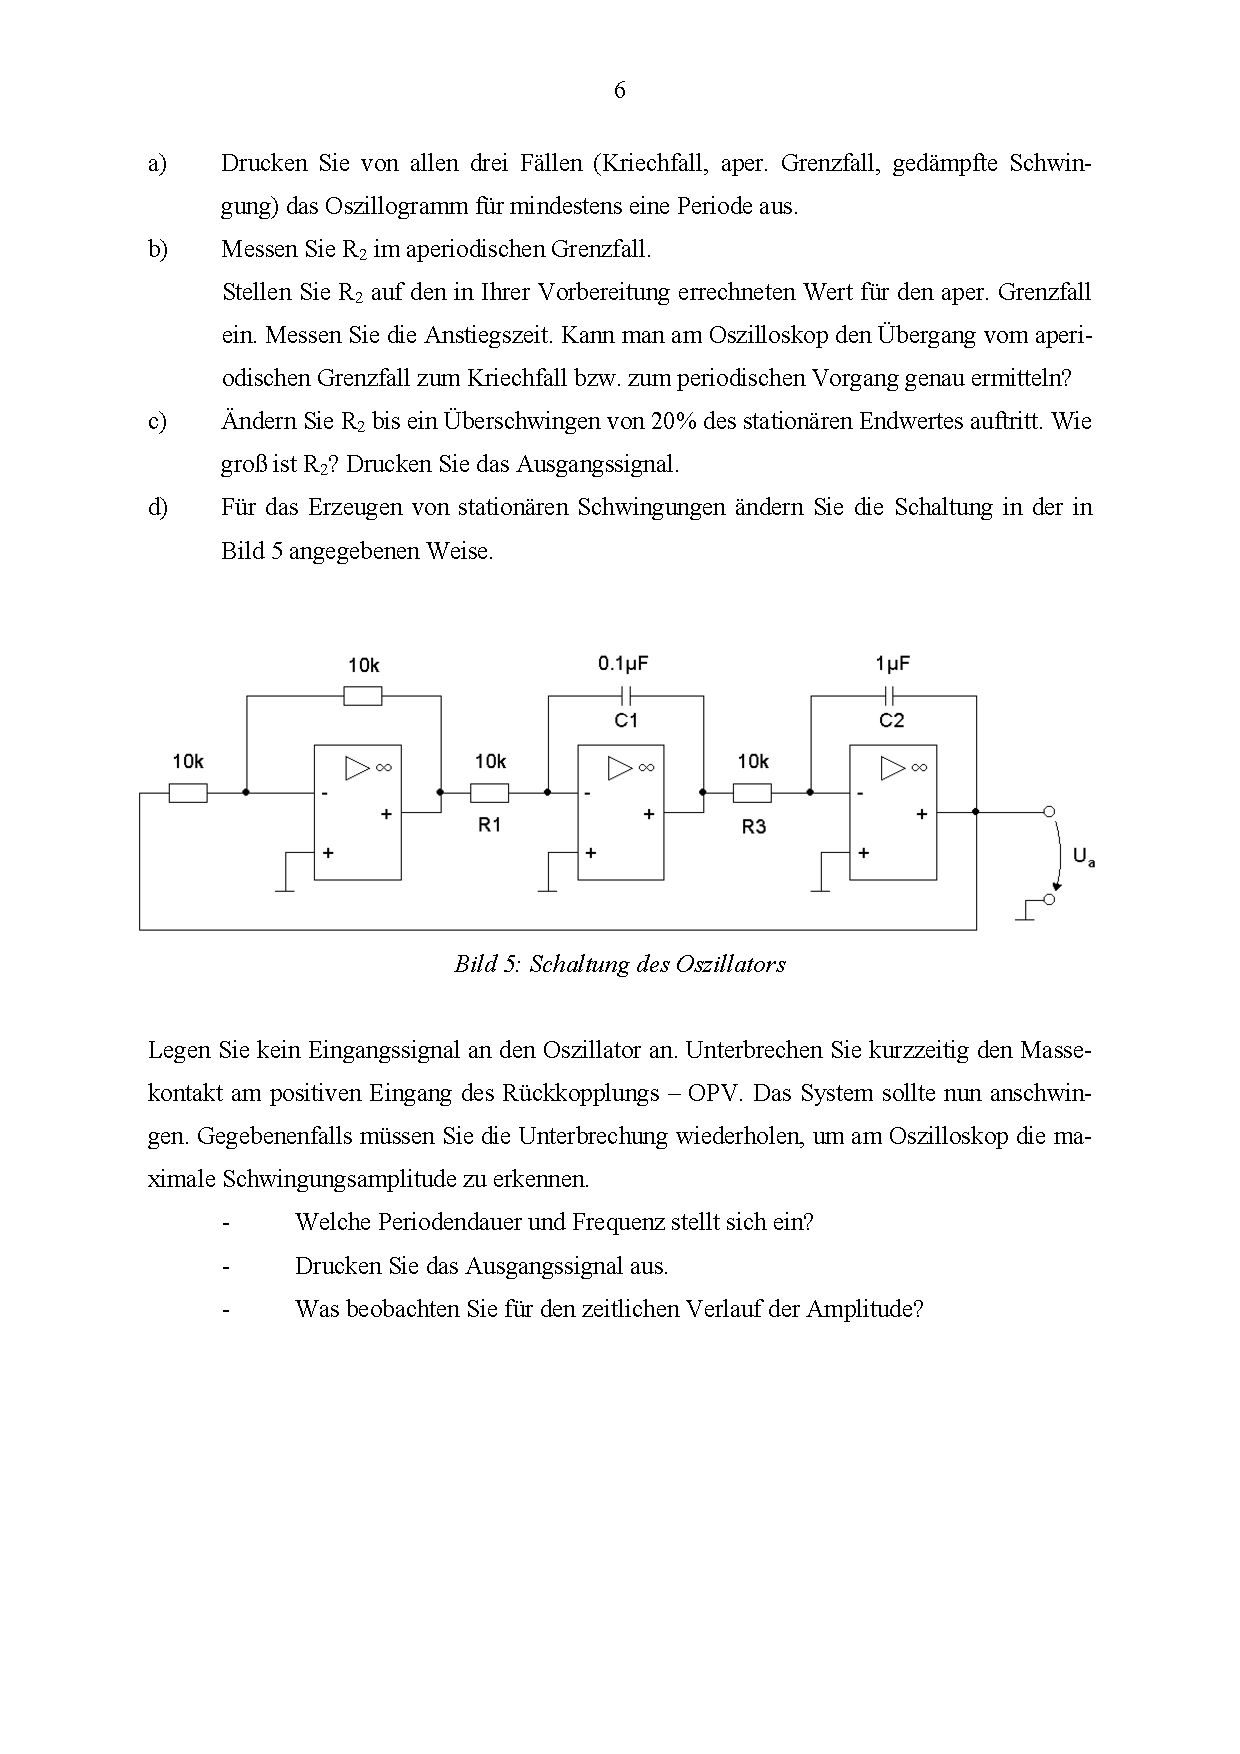
\includegraphics[width=1.0\textwidth]{Bilder/Grundubertragungsglieder im Zeitbereich (verschoben) 6}\newpage
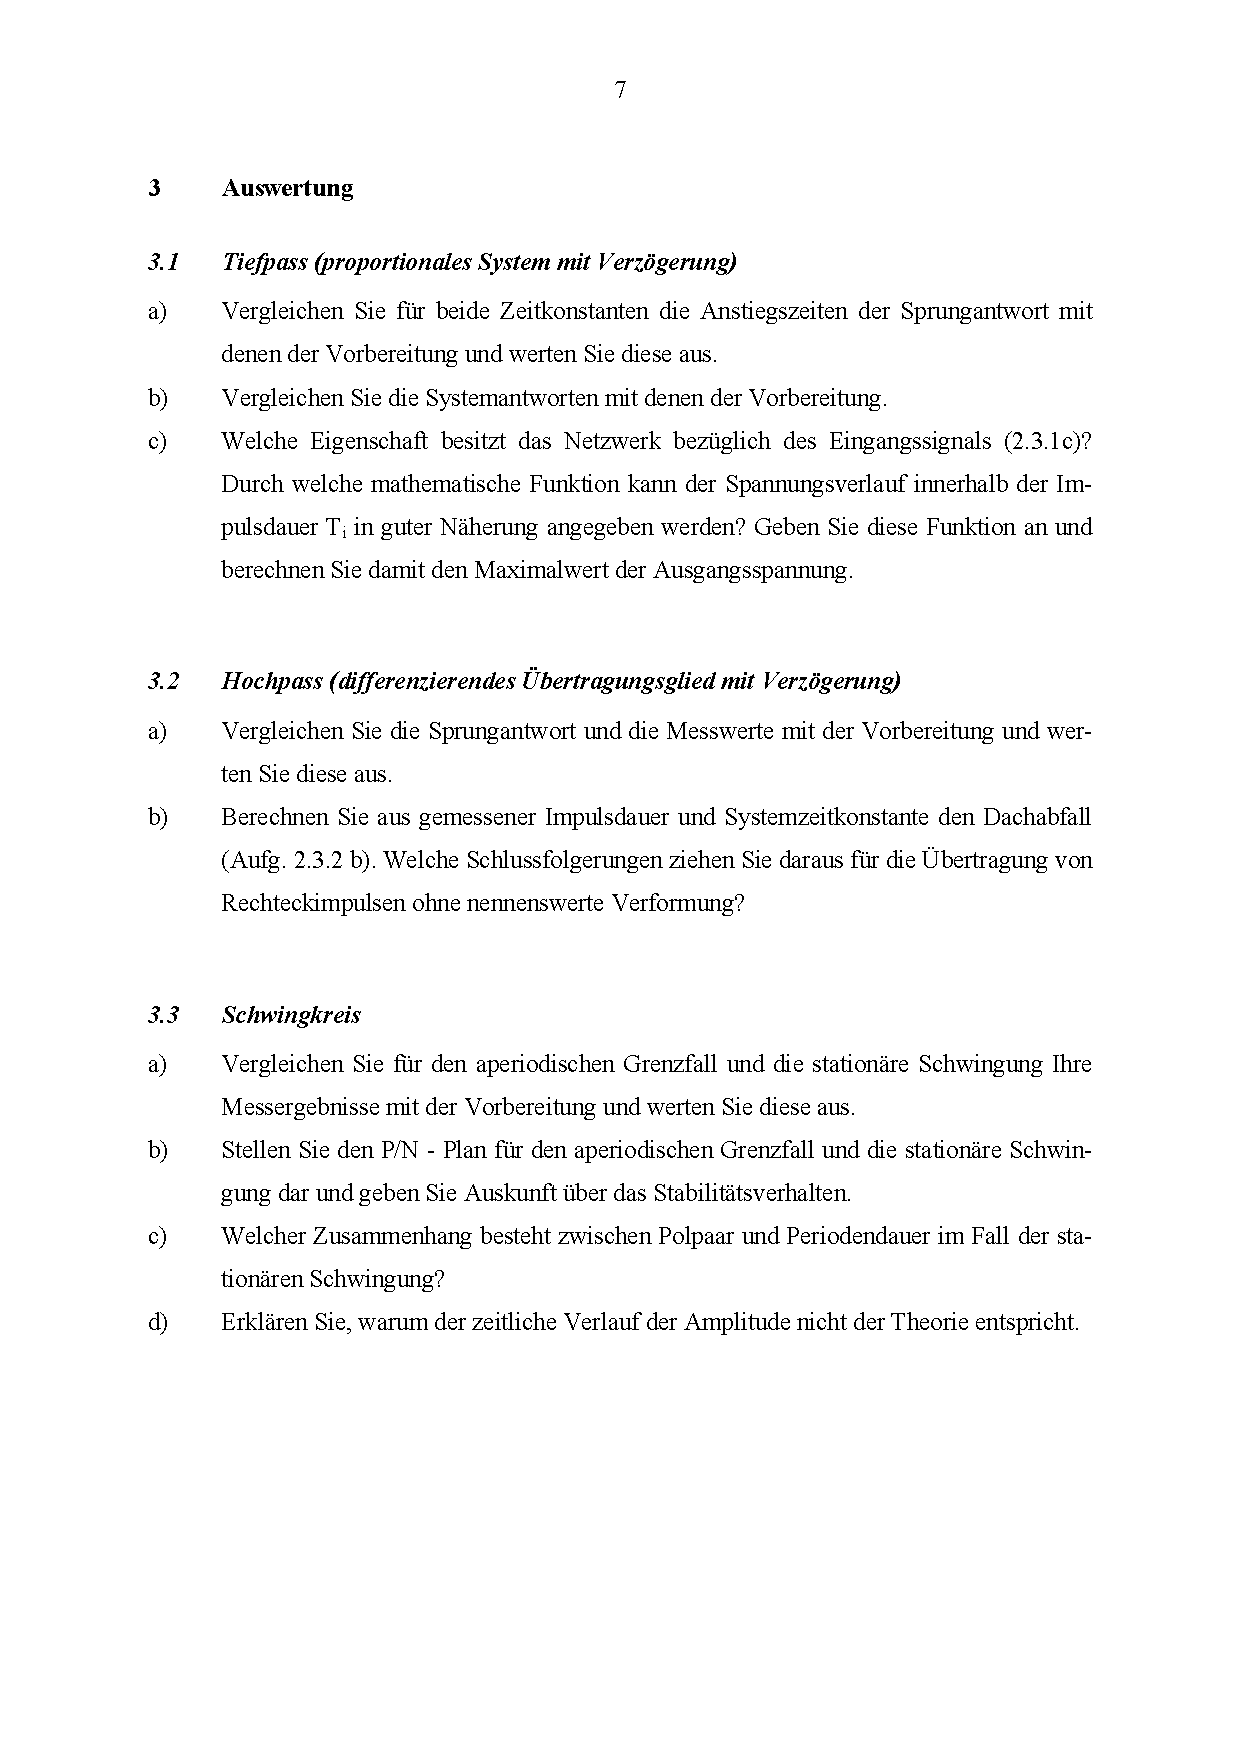
\includegraphics[width=1.0\textwidth]{Bilder/Grundubertragungsglieder im Zeitbereich (verschoben) 7}\newpage


\section{Vorbereitung des Versuches}

\subsection{Ziel und Abgrenzung des Versuches}

In diesem Versuch sollen die theoretischen Kenntnisse zu Ausgleichsvorgängen an 
einfachen Vierpolen vertieft werden. Es werden Sprung- und Rechteckimpulsantworten eines 
Tiefpasses, auch bezeichnet als proportionales System mit Verzögerung,eines Hochpasses, 
auch bezeichnet als differenzierenden System mit Verzögerung, und eines Schwingkreises untersucht.\\
\newline

\subsection{TheoretischeVoraussetzungen}

Wiederholen Sie in Vorbereitung auf diesen Versuch die Beschreibung 
zeitkontinuierlicher Systeme im Zeit- und Bildbereich.
\newline


\subsection{Vorbereitende Aufgaben}

\subsubsection{Begriffe}

Wie sind die Signalgrößen Anstiegs- und Abfallzeit, Dachabfall, Impulsdauer und Überschwingen definiert?\\
\newline%TODO
Wie sind die Systemantworten Übergangsfunktion und Sprungantwort definiert?\\
\newline%TODO

\subsubsection{Tiefpass (proportinales System mit Verzögerung)}

Ein proportionales System mit Verzögerung 1. Ordnung ist in Bild 1 dargestellt.\\
\begin{itemize}
\item a)    Geben  Sie  die  Übertragungsfunktion  $G(p)$,  die  Übertragungskonstante  KP und die Zeit-konstante T1 an.\\ 
\newline%TODO
\item b)    Ermitteln  Sie  die  Sprung-  und  Impulsantwort. Skizzieren  Sie  deren  qualitativen  Verlauf und tragen Sie die Zeitkonstante T1 in h(t) ein.\\ 
\newline%TODO
\item c)    Wie lang sind die Anstiegszeiten für einen Sprung bei $T_{ 1 }=100\mu s$ und $T1 = 1 ms$?\\ 
\newline%TODO
\item d)    Berechnen Sie R2 für die beiden Zeitkonstanten.\\ 
\newline%TODO
\item e)    Welche Impulsfolgefrequenz ist bei einem Tastgrad $k = 0,2$ und einer System-zeitkonstante $T1 = 1 ms$ zu wählen, um den Ausgleichsvorgang darzustellen\\
\newline%TODO
\end{itemize}

\subsubsection{Hochpass (differenzierendes Übertragungsglied mit Verzögerung)}

Ein differenzierendes Übertragungsglied mit Verzögerung 1. Ordnung ist in Bild 2 dargestellt.\\
Geben  Sie  die  Übertragungsfunktion $G(p)$,  die  Übertragungskonstante  KD und die Zeitkon-stante $T1$ an.\\ 
Ermitteln Sie die Sprungantwort und skizzieren Sie deren qualitativen Verlauf.\\ 
Wie lang ist die Abfallzeit der Sprungantwort bei einer Zeitkonstante $T1 = 1 ms$?\\ 
Nach welcher Zeit tritt ein Dachabfall von $10\%$ auf ?\\

\subsubsection{Schwingkreis}

Eine mögliche Realisierungsform des Schwingkreises ist in Bild 3 dargestellt.\\

Die Berechnung der Gesamtübertragungsfunktion erfolgt formal nach folgender Gleichung: \\
\newline
\begin{equation}
	\frac{ U_{ a }(p) }{ U_{ e }(p) } =\frac{ G_{ 1 }(p)*G_{ 2 }(p) }{ 1+G_{ 1 }(p)*G_{ 2 }(p)  }
\end{equation}
\newline
Elektronisch wird der Schwingkreis durch ein aktives RC-Filter mit einstellbarer Zeitkonstante
und Proportionalitätsfaktor sowie einem Integrierer realisiert.\\
Geben Sie die Gesamtübertragungsfunktion an, und berechnen Sie die Konstanten KP, KI und T1. 
Wandeln Sie die Gesamtübertragungsfunktion in die Form $G(p)=\frac{ 1 }{ p^{ 2 }T^{ 2 }+p2DT+1 }$ um, und geben Sie T und D allgemein an. 
Wie groß muss R2 sein, sodass bei diesem Schwingkreis der Kriechfall, der aperiodische Grenzfall oder ein 
abklingender periodischer Vorgang auftritt?\\
\newline%TODO
Ermitteln Sie mittels Übergangsfunktion die Anstiegszeit im 
aperiodischen Grenzfall. \\
Überlegen Sie, welches Rechtecksignal man am Eingang des Systems anlegen muss, um die 
Ausgleichsvorgänge anschaulich darzustellen zu können. Welchen Tastgrad muss man einstellen?\\
\newline%TODO 
Sollte die Impulsfolgefrequenz größer oder kleiner als die Eigenfrequenz des Systems mit periodischem Vorgang sein?\\
\newline%TODO
Wie ist R2 festzulegen, um eine stationäre Schwingung zu erhalten?\\
\newline%TODO 
Wie ändert sich durch Variation von R2 das Systemverhalten dieses Übertragungsgliedes?\\
\newline%TODO 
Welche Eigenfrequenz und Periodendauer hat dieser Schwingkreis?\\
\newline%TODO

\section{Durchführung des Versuchs}

\subsection{Versuchseinrichtung}

Analog – Board hps 3220 \\
Pulsgenerator PM5715 \\
Zweikanaloszilloskop PM3370B \\
Drucker Epson SQ2550\\

\subsection{Methodische Hinweise}

Lesen Sie zunächst die am Versuchsplatz ausliegende Kurzanleitung zur Einstellung des Pulsgenerators. \\
Beachten Sie, dass in Aufgabe 2.3 durch die OPV - Beschaltung eine Invertierung stattfindet. Berücksichtigen 
Sie dies bei der Einstellung des Oszilloskopes. Zur sicheren Abbildung ist das Oszilloskop extern aus dem 
Pulsgenerator zu triggern. Arbeiten Sie im Digital - Modus, um die Ergebnisse auch ausdrucken zu können. 
Drucken Sie das Ausgangssignal immer gemeinsam mit dem Eingangssignal des Systems in einem Bild aus. 
Koppeln Sie die Signale direkt mit dem Oszilloskop (DC – Modus).

\subsection{Aufgabenstellung}

\subsubsection{Tiefpass (proportinales System mit Verzögerung)}

Stellen Sie am Pulsgenerator eine Rechteckimpulsfolge mit einer Frequenz $f = 40 Hz$, einem Tastgrad 
$k = 0,2$ und positiven Impulsen von 1V Maximalspannung ein. 

\begin{itemize}
\item a) Stecken Sie einen Tiefpass mit einer Zeitkonstante $T1 = 1ms$. 
\begin{itemize}
	\item Messen Sie die Zeitkonstante, Anstiegszeit und Impulsdauer. 
	\item Drucken Sie das Ein- und Ausgangssignal aus.
\end{itemize}
\end{itemize} 
\begin{itemize}
	\item b) Verändern  Sie  die  Zeitkonstante auf  $100  \mu s$,  indem  Sie  den  Widerstand  $R2$ im Rückkoppelzweig 
			mit einen $1k \Omega Widerstand$ ersetzen. 
\begin{itemize}
	\item Messen Sie die Zeitkonstante, Anstiegszeit und Impulsdauer. 
	\item Drucken Sie das Ein- und Ausgangssignal aus. 
	\item Warum ändert sich der stationäre Endwert? 
\end{itemize}
\end{itemize}
\begin{itemize}
	\item c) Verringern  Sie  die  Impulsdauer  des  Eingangssignals  auf  $200 \mu s$.  Die  Zeitkonstante wird wieder auf $1 ms$ erhöht. 
\begin{itemize}
	\item Wie groß ist die maximale Spannung des Ausgangssignals? 
	\item Stellen Sie das Signal über zwei Perioden dar, und drucken Sie das Oszillogramm aus. 
\end{itemize}
\end{itemize}
\subsubsection{Hochpass (differenzierendes Übertragungsglied mit Verzögerung)}
Stecken Sie einen Hochpass mit einer Zeitkonstante von 1 ms.\\
\begin{itemize}
	\item a) Stellen Sie eine Impulsdauer von 5 ms ein. Behalten sie die Frequenz $f =40 Hz$ bei.
\begin{itemize}
\item Ermitteln Sie durch geeignete Messung aus dem Oszillogramm die Zeitkonstante des Systems, sowie die Abfallzeit $t_{f}$ der Sprungantwort. 
\item Drucken Sie die Sprungantwort, dargestellt über 10 ms (2ti), aus. 
\end{itemize}
\end{itemize}
\begin{itemize}
	\item b) Ändern Sie die Impulsdauer bis ein Dachabfall von $10\%$ auftritt.\\
\begin{itemize}
	\item Welche Impulsdauer hat das Eingangssignal?	
\end{itemize}
\end{itemize}
\subsubsection{Schwingkreis}
Bauen Sie ein rückgekoppeltes System nach Bild 4 auf.\\
Stellen Sie eine Rechteckimpulsfolge mit einer Frequenz von 10 Hz und einem Tastgrad $k = 0,5$ ein, um den Ausgleichsvorgang darzustellen.\\ 
Variieren Sie den Widerstand $R2$, um aperiodische und abklingende periodische Vorgänge zu erzeugen.\\
\begin{itemize}
\item 	a) Drucken Sie von allen drei Fällen (Kriechfall, aper. Grenzfall, gedämpfte Schwingung) das Oszillogramm für mindestens eine Periode aus. 
\item	b) Messen Sie R2 im aperiodischen Grenzfall. Stellen Sie R2 auf den in Ihrer Vorbereitung errechneten Wert für den aper. Grenzfall ein.
Messen Sie die Anstiegszeit. Kann man am Oszilloskop den Übergang vom aperi-odischen Grenzfall zum Kriechfall bzw. zum periodischen 
Vorgang genau ermitteln? 
\item 	c) Ändern Sie R2 bis ein Überschwingen von 20\% des stationären Endwertes auftritt. 
Wie groß ist R2? Drucken Sie das Ausgangssignal. 
\item	d) Für das Erzeugen von stationären Schwingungen ändern Sie die Schaltung in der in Bild 5 angegebenen Weise. 
\end{itemize}
\section{Auswertung}
\subsection{Tiefpass (proportinales System mit Verzögerung)}
\begin{itemize}
\item a) Vergleichen  Sie  für  beide  Zeitkonstanten die  Anstiegszeiten der Sprungantwort mit denen der Vorbereitung und werten Sie diese aus. 
\item b) Vergleichen Sie die Systemantworten mit denen der Vorbereitung. 
\item c) Welche Eigenschaft besitzt das Netzwerk bezüglich des Eingangssignals (2.3.1c)? Durch welche mathematische Funktion kann der Spannungsverlauf 
innerhalb der Impulsdauer Ti in guter Näherung angegeben werden? Geben Sie diese Funktion an und berechnen Sie damit den Maximalwert der Ausgangsspannung. 
\end{itemize}
\subsection{Hochpass (differenzierendes Übertragungsglied mit Verzögerung)}
\begin{itemize}
\item a) Vergleichen Sie die Sprungantwort und die Messwerte mit der Vorbereitung und werten Sie diese aus. 
\item b) Berechnen Sie aus gemessener Impulsdauer und Systemzeitkonstante den Dachabfall (Aufg. 2.3.2 b). Welche Schlussfolgerungen ziehen 
Sie daraus für die Übertragung von Rechteckimpulsen ohne nennenswerte Verformung?
\end{itemize}
\subsection{Schwingkreis}
\begin{itemize}
\item a) Vergleichen Sie für den aperiodischen Grenzfall und die stationäre Schwingung Ihre Messergebnisse mit der Vorbereitung und werten Sie diese aus. 
\item b) Stellen Sie den P/N - Plan für den aperiodischen Grenzfall und die stationäre Schwingung dar und geben Sie Auskunft über das Stabilitätsverhalten. 
\item c) Welcher Zusammenhang besteht zwischen Polpaar und Periodendauer im Fall der stationären Schwingung? 
\item d) Erklären Sie, warum der zeitliche Verlauf der Amplitude nicht der Theorie entspricht. 
\end{itemize}

